\documentclass[article,shortnames]{jss}
%%%%%%%%%%%%%%%%%%%%%%%%%%%%%%
%% declarations for jss.cls %%%%%%%%%%%%%%%%%%%%%%%%%%%%%%%%%%%%%%%%%%
%%%%%%%%%%%%%%%%%%%%%%%%%%%%%%

\usepackage{amssymb}
%% almost as usual
\author{Stefan R\"odiger$^{\ddag,\S}$\\Lausitz University of\\Applied Sciences\\ \& Charit\'e
	\And Thomas Friedrichsmeier$^{\ddag,\S}$\\Ruhr-University Bochum
	\AND Prasenjit Kapat\\The Ohio State University
	\And Meik Michalke\\Heinrich Heine University\\D\"usseldorf
}
\title{Supplement to:\linebreak 
  \pkg{RKWard} -- A Comprehensive Graphical User Interface and Integrated Development Environment for Statistical Analysis with \proglang{R}}

%% for pretty printing and a nice hypersummary also set:
\Plainauthor{Stefan R\"odiger, Thomas Friedrichsmeier, Prasenjit Kapat, Meik Michalke} %% comma-separated
\Plaintitle{RKWard -- A Comprehensive Graphical User Interface and Integrated Development Environment for Statistical Analysis with {R}} %% without formatting
\Shorttitle{\pkg{RKWard} a GUI for \proglang{R}} %% a short title (if necessary)

%% an abstract and keywords
\Abstract{
\pkg{RKWard} is a GUI to \proglang{R} with the objective to provide a 
portable and extensible \proglang{R} interface for both
basic and advanced statistical and graphical analysis. This supplement discusses 
in detail technical aspects of \pkg{RKWard} including the usage of the \pkg{KDE}/\pkg{Qt} software libraries which are the base of \pkg{RKWard}.
Statistical procedures and plots are implemented extendable plugin architecture in \pkg{RKWard}. 
This plugin architechture is based on \proglang{ECMAScript} (\proglang{JavaScript}), \proglang{R}, and XML. The general 
design is described and its application is exemplified on a t-test.
\newline
Disclaimer: This supplement was not part of the peer-review process of the Journal of Statistical Software.

\line(1,0){40}
\item$^{\ddag}$Equal contribution, $^{\S}$Corresponding authors
%%
}
\Keywords{cross-platform, GUI, integrated development environment, plugin, \proglang{R}}

\Plainkeywords{cross-platform, GUI, integrated development environment, plugin, R} %% without formatting
%% at \leftarrowst one keyword must be supplied


%% publication information
%% NOTE: Typically, this can be left commented and will be filled out by the technical editor
%% \Volume{13}
%% \Issue{9}
%% \Month{September}
%% \Year{2004}
%% \Submitdate{2004-09-29}
%% \Acceptdate{2004-09-29}

%% The address of (at least) one author should be given
%% in the following format:
\Address{
  Stefan R\"odiger\\
  Lausitz University of Applied Sciences\\
  Department of Bio-, Chemistry and Process Engineering\\
  AND\\
  Center for Cardiovascular Research (CCR)\\
  Charit\'e, Germany\\
  E-mail: \email{stefan\_roediger@gmx.de}\\
  E-mail: \email{rkward-devel@lists.sourceforge.net}\\
}

% \Address{
%  Prasenjit Kapat\\
%  Affiliation\\
%  Department\\
%  E-mail: \email{noname@here.org}
% }
% \Address{
%  Meik Michalke\\
%  Affiliation\\
%  Department\\
% }


%% for those who use Sweave please include the following line (with % symbols):
%% need no \usepackage{Sweave.sty}

%% end of declarations %%%%%%%%%%%%%%%%%%%%%%%%%%%%%%%%%%%%%%%%%%%%%%%

\begin{document}

%% include your article here, just as usual
%% Note that you should use the \pkg{}, \proglang{} and \code{} commands.
\newpage 
\section{Technical design}
\label{sec:technical}
This supplemt will give a compact overview of the key aspects of \pkg{RKWard}'s
development process and technical design. We will give slightly more attention to the details of the
plugin framework (see origial paper for further information) used in \pkg{RKWard}, since this is central to the extensibility of
\pkg{RKWard}.

\subsection{Development process}
\subsubsection[RKWard core and external plugins]{\pkg{RKWard} core and external plugins}
\label{sec:technical_processes_plugins}
Newly developed plugins are placed in a dedicated plugin map file.
Plugins in this map are not visible to the user by
default, but need to be enabled manually. Once the author(s) of a plugin
announces that they consider it stable, the plugin is subjected to a review for
correctness, style, and usability. The review status is tracked in the project
wiki. Currently at least one positive review is needed before the plugin is
allowed to be made visible by default, by moving it to an appropriate plugin
map.

The current development version adds support for downloading additional sets of
plugins, which are neither officially included nor supported by the
\pkg{RKWard} developers, from the internet.

\subsubsection{Automated testing}
\label{sec:technical_processes_automatedtesting}
A second requirement for new plugins is that each plugin must be accompanied by
at least one automated test. The automated testing framework in \pkg{RKWard} consists
of a set of \proglang{R} scripts which allow to run a plugin with specific GUI settings,
automatically\footnote{
  In the current development version, the scripts have been converted into a proper
  \proglang{R} package.
}. The resulting \proglang{R} code, \proglang{R} messages, and output are then compared
to a defined standard. Automated tests are run routinely after changes in the
plugin infrastructure, and before any new release.

The automated testing framework is also useful in testing some aspects of the
application which are not implemented as plugins, but this is currently limited
to very few basic tests.

\subsection{Asynchronous command execution}
\label{sec:technical_asynchronous}
One central design decision in the implementation of \pkg{RKWard} is that the
interface to the \proglang{R} engine operates asynchronously. The intention is to
keep the application usable to a high degree, even during the computation of
time-consuming analysis. For instance, while waiting for the estimation of a
complex model to complete, the user should be able to continue to use the GUI to
prepare the next analysis. Asynchronous command execution is also a prerequisite
for an implementation of the plot-preview feature (see Section~\ref{sec:plot_previews}). Commands
generated from plugins or user actions are placed in queue and are evaluated in
a separate thread in the order they were submitted\footnote{
    It is possible, and in some cases necessary, to enforce a different order of command execution in
    internal code. For instance, \pkg{RKWard} makes sure that no user command can
    potentially interfere while \pkg{RKWard} is loading the data of a \code{data.frame} for
    editing.
}. The asynchronous design implies that \pkg{RKWard} avoids relying on the
\proglang{R} engine during interactive use. This is one of several reasons for
the use of \proglang{ECMAScript} in plugins, instead of scripting using
\proglang{R} itself (see Sections~\ref{sec:technical_toolkit} and \ref{sec:technical_plugins}).
A further implication is that \pkg{RKWard} avoids querying information about the
existence and properties of objects in \proglang{R} interactively. Rather,
\pkg{RKWard} keeps a representation of \proglang{R} objects and their basic properties
(e.\,g., class and dimensions), which is used for the workspace browser (Section~\ref{sec:workspace_browser_object_viewer}),
object name completion, function argument hinting, and
other places. The object representation includes objects in all environments
in the search path, and any objects contained within these environments in a
hierarchical tree\footnote{
    Currently, environments of functions or formulas are not taken into account.
}. The representation of \proglang{R} objects is gathered
pro-actively. This has a notable impact on performance when loading packages.
Specifically, objects which would usually be ``lazy loaded'' only when needed \citep[see][]{Ripley2004} are
accessed in order to fetch information on their properties. This means the data
has to be loaded from disk; however, the memory is freed immediately after fetching
information on the object. Additionally, for packages with extremely large number of objects, \pkg{RKWard}
provides an option to exclude specific packages from scanning the object structures.

A further side-effect of the asynchronous threaded design is that there is
inherently a rather clear separation between the GUI code and the code making direct use
of the \proglang{R} application programming interface (API) (see also Figure~\ref{fig:design_sketch}). 
In the current development version, the evaluation
of \proglang{R} commands has even been moved into a separate process. Therefore in future releases it could 
be made possible to run GUI and \proglang{R} engine on different computers.

\begin{figure}[t!]
 \centering
 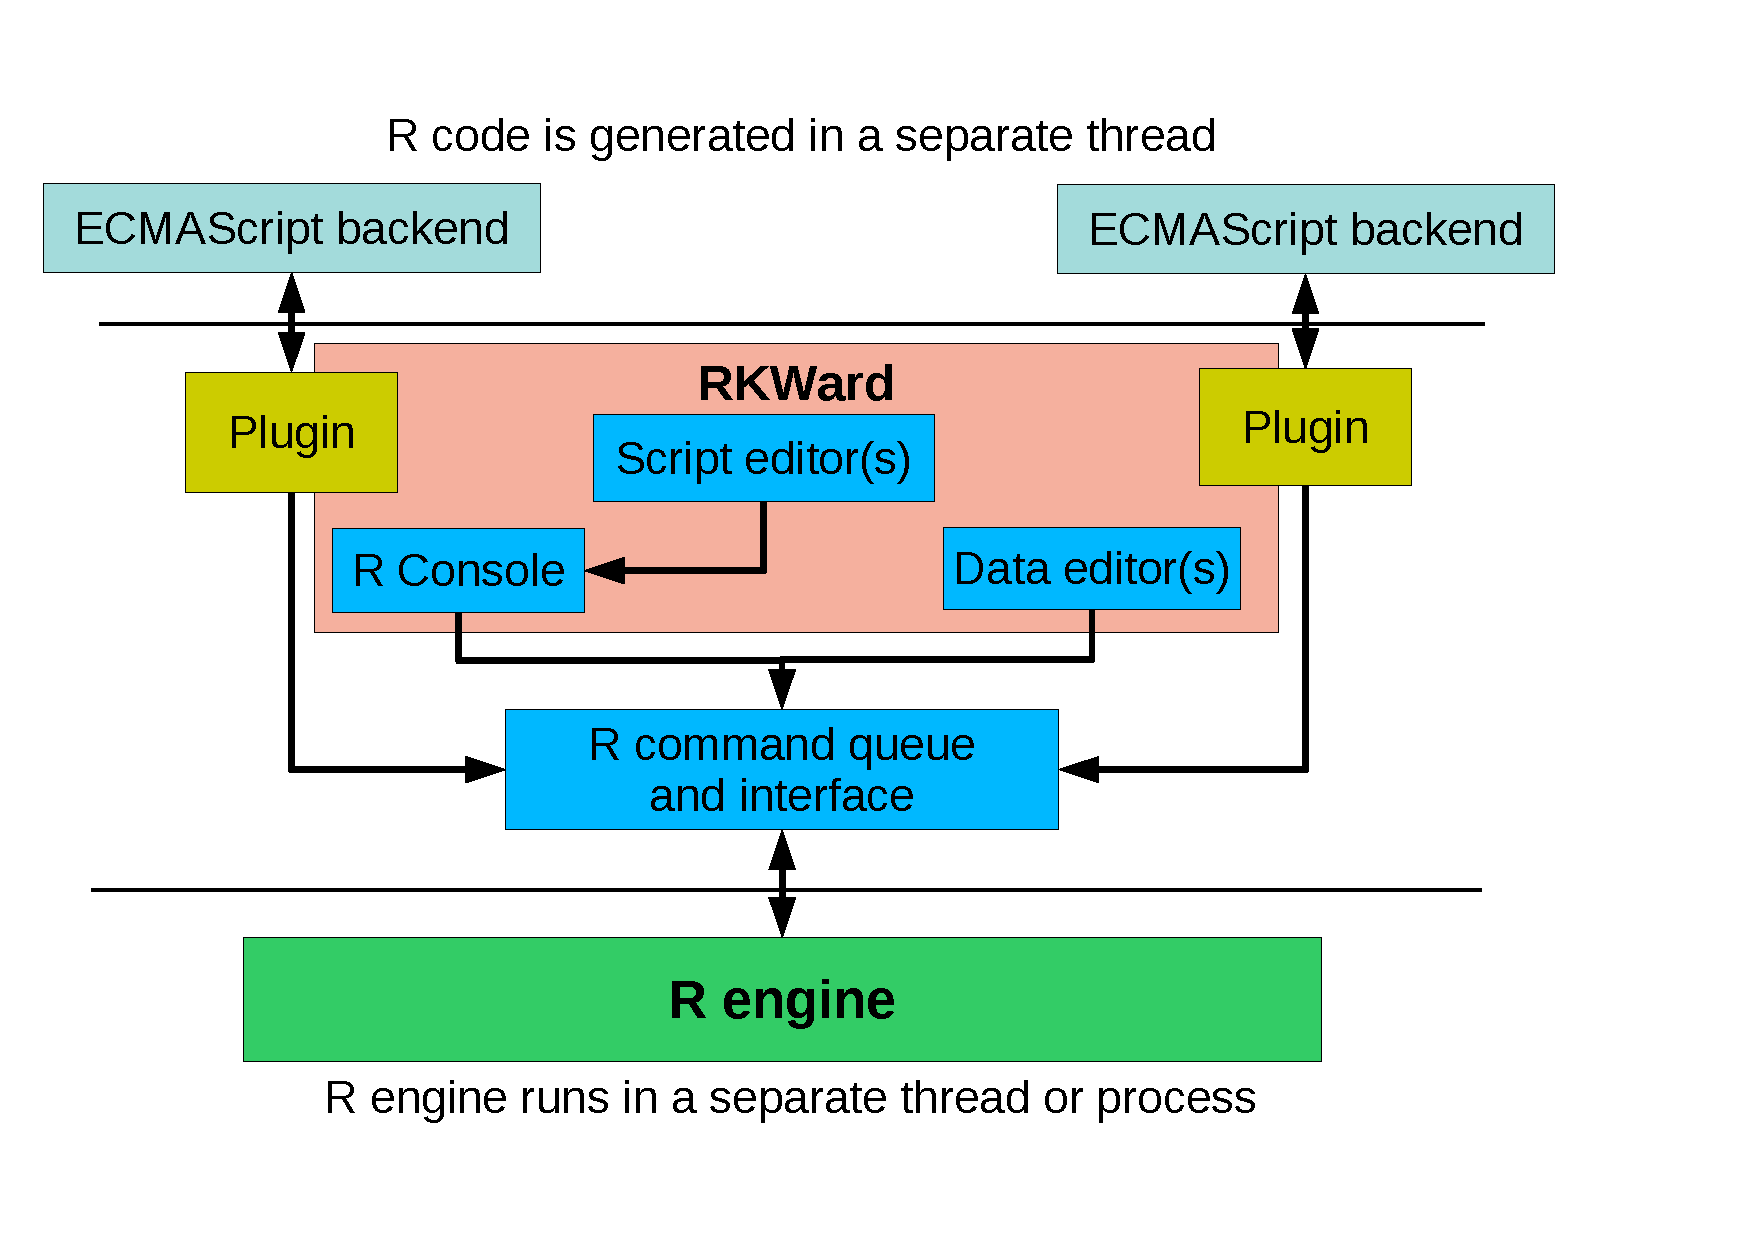
\includegraphics[clip=true,trim=0cm 2cm 0cm 0cm]{./figures/design_sketch.pdf}
 \caption{Technical design of \pkg{RKWard}. Only a few central components are visualized.
 All communication with the \proglang{R} engine is passed through a single interface living in the main application thread. The \proglang{R} engine itself
 runs in a separate thread (or in a separate process). 
 Separate threads are also used to generate \proglang{R} code from plugins.
}
 \label{fig:design_sketch}
\end{figure}

\subsection{Object modification detection}
\label{sec:technical_omd}
\pkg{RKWard} allows the user to run arbitrary commands in \proglang{R} at any time, even while
editing a \code{data.frame} or while selecting objects for analysis in a GUI dialog. Any user
command can potentially add, modify, or remove objects in \proglang{R}. \pkg{RKWard} tries to
detect such changes in order to always display accurate information in the
workspace browser, object selection lists, and object views. Beyond that,
detecting any changes is particularly important with respect to objects which
are currently being edited in the data editor (which provides an illusion
of in-place editing, see Section~\ref{sec:spreadsheet}). Here, it is necessary to synchronize
the data between \proglang{R} and the GUI in both directions.

For simplicity and performance, object modification detection is only
implemented for objects inside the ``global environment'' (including environments
inside the global environment), since this is where changes are typically done.
Currently, object modification detection is based on active bindings.
Essentially, any object which is created in the global environment is first
moved to a hidden storage environment, and then replaced with an active binding.
The active binding acts as a transparent proxy to the object in the storage
environment, which registers any write-access to the object\footnote{
    This is similar to the approach taken in the \pkg{trackObjs} package \citep{Plate2009}.
}.

The use of active bindings has significant performance implications when
objects are accessed very frequently. This is particularly notable where an
object inside the global environment is used as the index variable in a loop,
as illustrated by the following example. When control returns to the top level
prompt, after the first assignment, \code{i} will become subject to object modification
detection (i.\,e., it will be wrapped into an active
binding). The subsequent \code{for} loop will then run slow.

\begin{Code}
R> i <- 1
R> for (i in 1:100000) i + i
\end{Code}

In contrast, in the following example, \code{i} is a local object, and will not
be replaced by an active binding. Therefore the loop will run approximately as fast
as in a plain \proglang{R} session:

\begin{Code}
R> f <- function () {
R+    i <- 1
R+    for (i in 1:100000) i + i
R+ }
R> f ()
\end{Code}

Future versions of \pkg{RKWard} will try to avoid this performance problem. 
One approach that is currently under consideration is to simply perform
a pointer comparison of the \code{SEXP} records of objects in global environment with
their copies in a hidden storage environment. Due to the implicit sharing of
\code{SEXP} records \citep{RDCT2010a, RDCT2010b}, this should provide for a reliable
way to detect changes for most types of \proglang{R} objects, with comparatively low memory
and performance overhead. Special handling will be needed for environments and
active bindings.

\subsection{Choice of toolkit and implementation languages}
\label{sec:technical_toolkit}
In addition to \proglang{R}, \pkg{RKWard} is based on the \pkg{KDE} libraries, which are in turn based
on \pkg{Qt} \citep{perens1999}, and implemented mostly in \proglang{C++}. Compared to many competing libraries,
this constitutes a rather heavy dependency. Moreover, the \pkg{KDE} libraries are
still known to have portability issues especially on Mac OS X, and to some degree
also on the Microsoft Windows platform \citep{Jarvis2010}.

The major reason for choosing the \pkg{KDE} and \pkg{Qt} libraries was their 
many high level features which have allowed \pkg{RKWard} development to make quick
progress despite limited resources. Most importantly, the \pkg{KDE} libraries provide a
full featured text editor \citep{CullmannND} as a component which can be
seamlessly integrated into a host application using the KParts technology
\citep{Faure2000}. Additionally, another KPart provides HTML browsing capabilities in a
similarly integrated way. The availability of \pkg{KWord} \citep{KWord} as an
embeddable KPart might prove useful in future versions of \pkg{RKWard}, when better
integration with office suites will be sought.

Another technology from the \pkg{KDE} libraries that is important to the development
of \pkg{RKWard} is the ``XMLGUI'' technology
\citep{Faure2000}. This is especially helpful in providing an integrated GUI across
the many different kinds of document windows and tool views supported in \pkg{RKWard}.

Plugins in \pkg{RKWard} rely on XML\footnote{\url{http://www.w3.org/XML/}}
and \proglang{ECMAScript}\footnote{\url{http://www.ecmascript.org/}} (see Section~\ref{sec:technical_plugins}). XML is not
only well suited to describe the layout of the GUI of plugins, but simple
functional logic can also be represented \citep[see also][]{Visne2009}. \proglang{ECMAScript} was
chosen for the generation of \proglang{R} commands within plugins, in particular due to its
availability as an embedded scripting engine inside the \pkg{Qt} libraries. While at
first glance \proglang{R} itself would appear as a natural choice of scripting language as
well, this would make it impossible to use plugins in an asynchronous way.
Further, the main functional requirement in this place is the manipulation and
concatenation of text strings. While \proglang{R} provides support for this, concatenating
strings with the \code{+}-operator, as available in \proglang{ECMAScript}, allows for a much
more readable way to perform such basic text manipulation.

\subsection{On-screen graphics windows}
\label{sec:technical_graphics}
Contrary to the approach used in \pkg{JGR} \citep{JGR2010}, \pkg{RKWard} does
not technically provide a custom on-screen graphics device. \pkg{RKWard} detects when
new graphics windows are created via calls to \code{X11()} or \code{windows()}. These windows
are then ``captured'' in a platform dependent way (based on the XEmbed \citep{Ettrich2002} protocol
for \pkg{X11}, or reparenting for the Microsoft Windows platform). An \pkg{RKWard} menu bar and a
toolbar is then added to these windows to provide added functionality. While
this approach requires some platform dependent code, any corrections or
improvements made to the underlying \proglang{R} native devices will automatically be
available in \pkg{RKWard}.

A recent addition to the on-screen device is the ``plot history'' feature which
adds a browsable list of plots to the device window. Since \pkg{RKWard} does not use a
custom on-screen graphics device, this feature is implemented in a package
dependent way. For example, as of this writing, plotting calls that use either
the ``standard graphics system'' or the ``\pkg{lattice} system'' can be added to the plot
history; other plots are drawn but not added. The basic procedure is to identify
changes to the on-screen canvas and record the existing plot before a new plot
wipes it out. A single global history for the recorded plots is maintained
which is used by all the on-screen device windows. This is similar to the
implementation in \proglang{Rgui.exe} (Microsoft Windows), but unlike the one in \proglang{Rgui.app} 
(Mac OS X). Each such device window points to a position in the history
and behaves independently when recording a new plot or deleting an existing
one.

The \pkg{lattice} system is implemented by inserting a hook in the \code{print.lattice()}
function. This hook retrieves and stores the \code{lattice.status} object from the
\code{lattice:::.LatticeEnv} environment, thereby making \code{update()} calls on trellis
objects \citep[see also][]{Sarkar2008} transparent to the user. Any recorded trellis object is then replayed
using \code{plot.lattice()}, bypassing the recording mechanism. The standard graphics
system, on the other hand, is implemented differently because the hook in
\code{plot.new()} is ineffective for this purpose. A customized function is overloaded
on \code{plot.new()} which stores and retrieves the existing plot, essentially, using
\code{recordPlot()} and replays them using \code{replayPlot()}.

The actual plotting calls are tracked using appropriate \code{sys.call()} commands in
the hooks. These call strings are displayed as a drop-down menu on the toolbar
for non-sequential browsing (see Figure~\ref{fig:plot_history}) providing a very intuitive browsing
interface unlike the native implementations in \code{windows()} and \code{quartz()} devices.


\subsection{Internationalization}
\label{sec:technical_internationalization}
Currently strings in the main application are translated to varying extents in
Czech (cs), Catalan (ca), Spanish (es), German (de), Chinese (zh\_CN), Turkish
(tr), Polish (pl), Italian (it), French (fr), Greek (el), and Danish (da).
Translatable strings are to be found under po/*.po in the sources. These files
can conveniently be edited with front-ends like Lokalize\footnote{\url{http://i18n.kde.org/tools/}}. 

Plugins and help pages in \pkg{RKWard} are not translatable at the time of this
writing. While it will be technically possible to include the respective strings in
message catalogs, this is currently not implemented in \pkg{RKWard}. Similarly, any
output generated by \proglang{R} functions defined for \pkg{RKWard} is currently not
translatable. Again, however, there is no technical barrier with respect to
internationalization of \proglang{R} code, as discussed by \cite{Ripley2005a},
and it is planned to make \pkg{\pkg{RKWard}} fully translatable in future versions.

\bibliography{sources}
\end{document}
